\section{Lezione 2: Operazioni sulle
matrici}\label{lezione-2-operazioni-sulle-matrici}

Un \textbf{immagine raster} può essere \textbf{rappresentata} da una
\textbf{matrice}. Su una immagine \textbf{possono essere fatte tutte} le
\textbf{operazioni} che si possono fare sulle \textbf{matrici}, ma non è
detto che tali operazioni abbiano un senso logico, ad esempio cosa vuol
dire moltiplicare due immagini a un punto di vista visivo? Noi useremo
le operazioni matriciali come base per operazioni più complesse.

Quando faremo l'operazione di prodotto tra due matrici non useremo la
regola del riga per colonna, ma piuttosto il \textbf{punto a punto}
degli elementi corrispondenti. In questo modo:

\[
 \begin{bmatrix}1 & 0 & 2 \\-1 & 3 & 1 \\\end{bmatrix} \cdot \begin{bmatrix}3 & 1 \\2 & 1\\1 & 0 \\\end{bmatrix}= \begin{bmatrix}5 & 1 \\4 & 2 \\\end{bmatrix}
\]

\subsubsection{\texorpdfstring{Neighborhood
\(N_p\)}{Neighborhood N\_p}}\label{neighborhood-n_p}

\begin{itemize}
\item
  I vicini 4 connessi in un dato pixel sono quelli alla sua destra, alla
  sua sinistra, quelli sopra e quelli sotto

  \begin{figure}
  \centering
  \pandocbounded{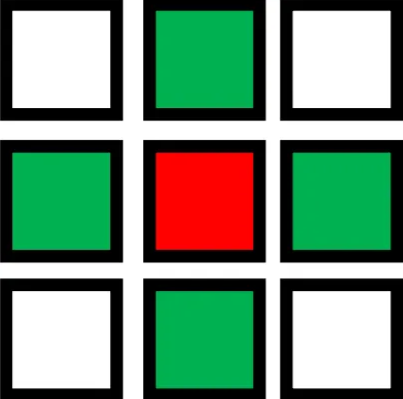
\includegraphics[keepaspectratio,alt={image.png}]{Lezione 2 Operazioni sulle matrici/8bfbb717-881f-4887-907b-6fc97e5348f6.png}}
  \caption{image.png}
  \end{figure}
\item
  I vicini 8 connessi sono quelli 4 connessi a cui si aggiungono i 4
  pixel in diagonale

  \begin{figure}
  \centering
  \pandocbounded{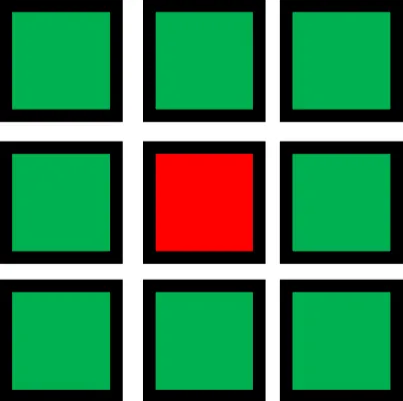
\includegraphics[keepaspectratio,alt={image.png}]{Lezione 2 Operazioni sulle matrici/e331fe04-cce2-432d-825c-90a41a51e4c3.png}}
  \caption{image.png}
  \end{figure}
\end{itemize}

\subsubsection{Operazioni affini}\label{operazioni-affini}

Si tratta di una \textbf{classe di operazioni} delle immagini che non
producono la variazione del valore del \textbf{pixel} ma ne
\textbf{determinano} solamente la \textbf{nuova posizione}. Esse sono le
operazioni di \textbf{identità, la rotazione, la traslazione, lo
scaling, lo shear.}

Le operazioni affini possono essere definite con una \textbf{matrice
3x3} \textbf{chiamata T}. La forma più comune è la definizione tramite
matrice.

\subsubsection{Forward mapping}\label{forward-mapping}

Il forward mapping è un metodo in cui:

\begin{itemize}
\tightlist
\item
  prendi ogni pixel dell'immagine in input
\item
  lo trasformi con una formula matematica
\item
  scopri dove va a finire nell'immagine di output
\end{itemize}

I pixel di input vengono definiti dalle coordinate \((v, \space w)\),
mentre quelli di output dalle coordinate \((x, \space y)\). Infine, come
detto prima, T è la matrice affine che descrive le operazioni affini di
trasformazione (traslazione, rotazione, scala, ecc\ldots).

In pratica: T dice come spostare i pixel.

Per ottenere il valore, basta utilizzare la formula:
\([x \space y \space 1] = [v \space w \space 1] \cdot T\)

Cosa significa? Prendi in input il pixel alle coordinate
\((v, \space w)\), lo scrivi come vettore \([v \space w \space 1]\), lo
moltiplichi per la matrice T e ottieni la nuova posizione
\((x, \space y)\).

Il numero 1 serve per poter includere le operazioni di traslazione.

Passo passo:

\begin{itemize}
\tightlist
\item
  scorri tutti i pixel dell'immagine di input
\item
  per ogni pixel \((v, \space w)\):

  \begin{itemize}
  \tightlist
  \item
    applichi la trasformazione
  \item
    calcoli \((x, \space y)\)
  \end{itemize}
\item
  metti il valore del pixel di input nella posizione \((x, \space y)\)
  dell'immagine di input
\end{itemize}

\textbf{Esempio concreto:}

Immagina una traslazione a destra di 10 pixel. Sappiamo che l'asse
orizzontale è x, dunque:

\begin{itemize}
\tightlist
\item
  pixel di input \((v = 5, \space w = 7)\)
\item
  trasformazione ``+10 su x''
\end{itemize}

Risultato

\begin{itemize}
\tightlist
\item
  pixel di output: (x = 15, y = 7)
\end{itemize}

Hai preso un pixel e gli hai detto dove andare.

Aggiungendo l'\textbf{1}, stiamo praticamente portando il nostro pixel
2D in uno spazio 3D, ma lo appoggiamo su un ``vassoio'' che si trova
all'altezza \(z = 1\).

\subsubsection{\texorpdfstring{La ``Mappa'' della Matrice Affine
\(3 \times 3\)}{La ``Mappa'' della Matrice Affine 3 \textbackslash times 3}}\label{la-mappa-della-matrice-affine-3-times-3}

In questa tabella vedi cosa controlla ogni cella. Ricorda che le colonne
decidono il risultato finale (x o y), mentre le righe decidono quale
dato in input andare a pescare (v, w o l'1 delle coordinate omogenee).

\(T = \begin{pmatrix}
\color{blue}{s_x \text{ (Scala X)}} & \color{green}{r \text{ (Ruota)}} & 0 \\
\color{green}{r \text{ (Ruota)}} & \color{blue}{s_y \text{ (Scala Y)}} & 0 \\
\color{red}{t_x \text{ (Sposta X)}} & \color{red}{t_y \text{ (Sposta Y)}} & 1
\end{pmatrix}\)

Prima colonna = x Seconda colonna = y Terza colonna = ``colonna di
servizio per le coordinate omogenee sulla traslazione''

\href{Lezione\%202\%20Operazioni\%20sulle\%20matrici/Svolgimento\%20esercizi\%202d11cf23380e80b6b137f81c6d70ed5a.md}{Svolgimento
esercizi}

\subsubsection{Inverse mapping}\label{inverse-mapping}

Abbiamo visto il forward mapping, l'unico problema causato da questi
straordinari calcoli è che lasciano dei buchi sull'immagine in output.

\begin{figure}
\centering
\pandocbounded{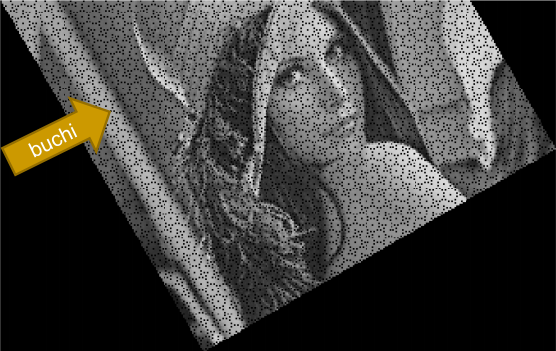
\includegraphics[keepaspectratio,alt={image.png}]{Lezione 2 Operazioni sulle matrici/image.png}}
\caption{image.png}
\end{figure}

\begin{figure}
\centering
\pandocbounded{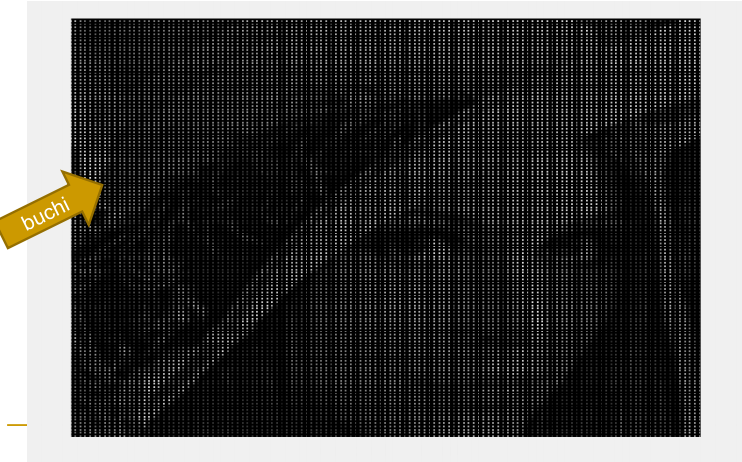
\includegraphics[keepaspectratio,alt={image.png}]{Lezione 2 Operazioni sulle matrici/image 1.png}}
\caption{image.png}
\end{figure}

L'\textbf{Inverse Mapping} è la strategia più utilizzata
nell'elaborazione delle immagini perché risolve in modo elegante i
problemi che abbiamo visto con il Forward Mapping (come i ``buchi'' o
l'effetto ``sale e pepe'').

\textbf{1. L'Algoritmo}

\begin{enumerate}
\def\labelenumi{\arabic{enumi}.}
\tightlist
\item
  \textbf{Crea} una griglia vuota per l'immagine di output.
\item
  \textbf{Scansiona} ogni pixel (x, y) della nuova immagine.
\item
  \textbf{Applica la Matrice Inversa} \(T^{-1}\) per trovare le
  coordinate originali (v, w).
\item
  \textbf{Preleva il colore} dalla posizione (v, w) dell'immagine
  originale.
\item
  \textbf{Copia} il colore nella posizione (x, y) dell'output
\end{enumerate}

\textbf{Tabella Rapida delle Trasformazioni Inverse}

{\def\LTcaptype{none} % do not increment counter
\begin{longtable}[]{@{}
  >{\raggedright\arraybackslash}p{(\linewidth - 4\tabcolsep) * \real{0.3333}}
  >{\raggedright\arraybackslash}p{(\linewidth - 4\tabcolsep) * \real{0.3333}}
  >{\raggedright\arraybackslash}p{(\linewidth - 4\tabcolsep) * \real{0.3333}}@{}}
\toprule\noalign{}
\begin{minipage}[b]{\linewidth}\raggedright
Operazione
\end{minipage} & \begin{minipage}[b]{\linewidth}\raggedright
Se l'andata (T) è\ldots{}
\end{minipage} & \begin{minipage}[b]{\linewidth}\raggedright
L'inversa (\(T^{-1}\)) sarà\ldots{}
\end{minipage} \\
\midrule\noalign{}
\endhead
\bottomrule\noalign{}
\endlastfoot
Traslazione & Sposta di +10 & Sposta di -10 \\
Scalatura & Ingrandisce di (x2) & Rimpicciolisce di (x0.5) \\
Rotazione & Ruota di \(\theta\) & Ruota di \textbf{\(\theta\)}
antiorario (Trasposta) \\
\end{longtable}
}

\href{Lezione\%202\%20Operazioni\%20sulle\%20matrici/Esercizi\%20Guida\%20(Svolti)\%202d11cf23380e80c297ccda1d7c4d84ad.md}{Esercizi
Guida (Svolti)}

\subsubsection{Interpolazione}\label{interpolazione}

Nel corso delle trasformazioni, potrebbero esserci dei valori di pixel
che non sono mai individuati dalle formule. Per essi si applica un
\textbf{processo di interpolazione}. Ossia il processo che,
\textbf{partendo da dati reali, stima i dati non conosciuti}.
L'interpolazione non comporta un miglioramento della qualità, ma
piuttosto ci fornisce dei valori ignoti mancanti stimandoli da valori
reali.

\subsubsection{Zooming}\label{zooming}

L'interpolazione è effettuata anche nei processi di zooming.

Se parliamo di \textbf{\emph{Zooming In}}, in 2x vuol dire che le
dimensioni dell'immagine verranno raddoppiate. Parlando di uno zoom 2x
in una matrice m x n allora diverrà 2m x 2n, ciò indica che il totale di
pixel verrà quadruplicato. Ovviamente ci sono altri tipi di scala nello
zooming, e non solo 2x.

\begin{figure}
\centering
\pandocbounded{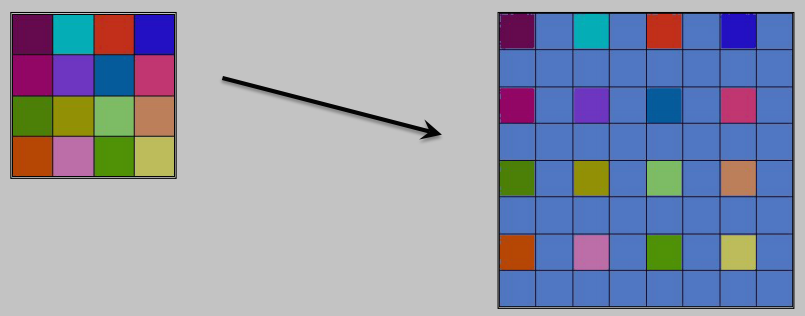
\includegraphics[keepaspectratio,alt={Zooming In 2x}]{Lezione 2 Operazioni sulle matrici/image 2.png}}
\caption{Zooming In 2x}
\end{figure}

Zooming In 2x

Dopo aver posizionato i valori già noti, occorre stimare i valori nelle
zone vuote.

\subsubsection{Vari tipi di
interpolazione}\label{vari-tipi-di-interpolazione}

\begin{itemize}
\tightlist
\item
  \textbf{Nearest neighbor (o replication)}
\item
  \textbf{Bilinear}
\item
  \textbf{Bicubic}
\end{itemize}

\begin{figure}
\centering
\pandocbounded{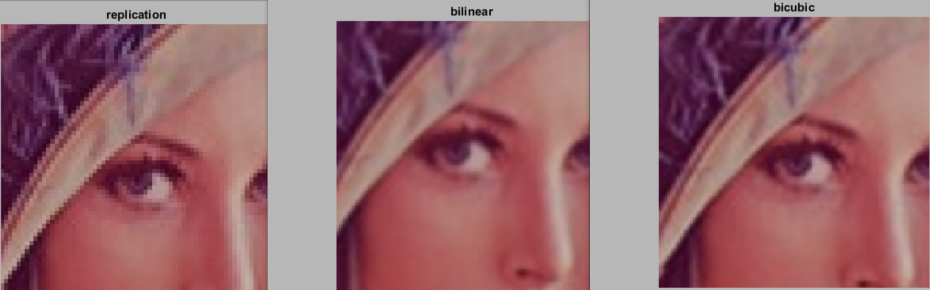
\includegraphics[keepaspectratio,alt={image.png}]{Lezione 2 Operazioni sulle matrici/image 3.png}}
\caption{image.png}
\end{figure}

\subsubsection{Nearest neighbor /
Replication}\label{nearest-neighbor-replication}

L'interpolazione \textbf{nearest neighbor} per le immagini funziona
\textbf{copiando il valore del pixel più vicino ai nuovi pixel creati}
quando si ingrandisce una matrice di pixel.

Pensa ad un'immagine che puoi rappresentare come una~\textbf{matrice di
pixel}, dove ogni elemento della matrice ha un valore che rappresenta il
colore o l'intensità del pixel. Se
vuoi~\textbf{ridimensionare}~l'immagine (ad esempio ingrandirla), hai
bisogno di ``inventare'' nuovi pixel che riempiano lo spazio tra quelli
originali.

Supponiamo di voler zoomare un'immagine di dimensione 2x2 in 4x4.

{\def\LTcaptype{none} % do not increment counter
\begin{longtable}[]{@{}ll@{}}
\toprule\noalign{}
A & B \\
\midrule\noalign{}
\endhead
\bottomrule\noalign{}
\endlastfoot
C & D \\
\end{longtable}
}

Quando espandi a una matrice 4x4, ci saranno nuovi ``spazi vuoti'' in
mezzo che devono essere riempiti. Con il metodo nearest neighbor, ogni
nuovo pixel viene semplicemente~\textbf{riempito copiando il valore del
pixel più vicino}~della matrice originale.

La matrice ingrandita 4x4 con nearest neighbor potrebbe diventare:

{\def\LTcaptype{none} % do not increment counter
\begin{longtable}[]{@{}llll@{}}
\toprule\noalign{}
A & A & B & B \\
\midrule\noalign{}
\endhead
\bottomrule\noalign{}
\endlastfoot
A & A & B & B \\
C & C & D & D \\
C & C & D & D \\
\end{longtable}
}

Questo fa sì che le aree dei nuovi pixel siano
piuttosto~\textbf{squadrate}~e non fluide, perché non c'è una
transizione graduale tra i colori. Questo può creare un effetto
a~\textbf{blocchi}, soprattutto se l'immagine viene ingrandita molto.

\subsubsection{Bilineare}\label{bilineare}

L'interpolazione bilineare utilizza i quattro pixel più vicini al punto.
Supponendo di avere le coordinate \((x,y)\) della posizione a cui
assegnare un nuovo valore di intensità, e supponendo che \(v(x,y)\)
equivalga al valore stesso dell'intensità, si può utilizzare
un'equazione:

\[
v(x,y) = ax + by +cxy+d
\]

Dove \(a\), \(b\), \(c\) e \(d\), ossia i \textbf{quattro coefficienti}
vengono \textbf{determinati} utilizzando i \textbf{valori di intensità}
dei \textbf{quattro pixel} noti \textbf{attorno al punto}.

E \((x, y)\) rappresenta le coordinate della posizione dove vuoi stimare
il valore dell'intensità.

I quattro coefficienti~\(a\), \(b\), \(c\) e \(d\) vengono calcolati
risolvendo un~\textbf{sistema di quattro equazioni}. Queste equazioni
derivano dai valori di intensità dei quattro pixel noti che circondano
il punto~ . Quindi, il valore di intensità nel nuovo punto dipende da
una combinazione ponderata di questi quattro pixel.

Determinare i coefficienti \(a\), \(b\), \(c\), \(d\) nella formula
dell'interpolazione bilineare: \(v(x, y) = ax + by + cxy + d\)

\subsubsection{Passo 1: Identificare i Valori di
Intensità}\label{passo-1-identificare-i-valori-di-intensituxe0}

Abbiamo i seguenti valori di intensità associati alle coordinate:

\begin{itemize}
\tightlist
\item
  \(V(1, 1) = 1\)
\item
  \(V(1, 3) = 2\)
\item
  \(V(3, 1) = 6\)
\item
  \(V(3, 3) = 7\)
\end{itemize}

\subsubsection{Passo 2: Costruire le
Equazioni}\label{passo-2-costruire-le-equazioni}

Utilizziamo i valori di intensità per costruire un sistema di equazioni.
Ogni equazione corrisponde a un punto noto e ci permette di esprimere le
intensità in funzione dei coefficienti \(a\), \(b\), \(c\), \(d\).

\subsubsection{\texorpdfstring{Equazione per il Punto
\((0, 0)\)}{Equazione per il Punto (0, 0)}}\label{equazione-per-il-punto-0-0}

\begin{enumerate}
\def\labelenumi{\arabic{enumi}.}
\tightlist
\item
  \textbf{Punto}: \((0, 0)\)

  \begin{itemize}
  \tightlist
  \item
    Questo punto corrisponde a \(V(1, 1) = 1\).
  \item
    Sostituendo nella formula:
    \(v(0, 0) = a(0) + b(0) + c(0)(0) + d = d\)
  \item
    Quindi abbiamo: \(d = 1\)
  \end{itemize}
\end{enumerate}

\subsubsection{Equazione per il Punto (1,
0)}\label{equazione-per-il-punto-1-0}

\begin{enumerate}
\def\labelenumi{\arabic{enumi}.}
\tightlist
\item
  \textbf{Punto}: \((1, 0)\)

  \begin{itemize}
  \tightlist
  \item
    Questo punto corrisponde a \(V(1, 3) = 2.\)
  \item
    Sostituendo nella formula:
    \(v(1, 0) = a(1) + b(0) + c(1)(0) + d = a + d\)
  \item
    Sostituiamo il valore di \(d = 1\): \(a + 1 = 2\)
  \item
    Risolvendo: \(a = 2 - 1 = 1\)
  \end{itemize}
\end{enumerate}

\subsubsection{Equazione per il Punto (0,
1)}\label{equazione-per-il-punto-0-1}

\begin{enumerate}
\def\labelenumi{\arabic{enumi}.}
\tightlist
\item
  \textbf{Punto}: \((0, 1)\)

  \begin{itemize}
  \tightlist
  \item
    Questo punto corrisponde a \(V(3, 1) = 6\).
  \item
    Sostituendo nella formula:
    \(v(0, 1) = a(0) + b(1) + c(0)(1) + d = b + d\)
  \item
    Sostituiamo il valore di \(d = 1\): \(b + 1 = 6\)
  \item
    Risolvendo: \(b = 6 - 1 = 5\)
  \end{itemize}
\end{enumerate}

\subsubsection{Equazione per il Punto (1,
1)}\label{equazione-per-il-punto-1-1}

\begin{enumerate}
\def\labelenumi{\arabic{enumi}.}
\tightlist
\item
  \textbf{Punto}: \((1, 1)\)

  \begin{itemize}
  \tightlist
  \item
    Questo punto corrisponde a \(V(3, 3) = 7\).
  \item
    Sostituendo nella formula:
    \(v(1, 1) = a(1) + b(1) + c(1)(1) + d = a + b + c + d\)
  \item
    Sostituiamo i valori trovati per \(a\), \(b\), e \(d\):

    \begin{itemize}
    \tightlist
    \item
      Con \(a=1\), \(b=5\), e \(d=1\):
    \item
      Quindi: \(v(1, 1)=a+b+c+d=7\) Diventando: \(1 + 5 + c + 1 = 7\)
      Risolvendo: \(c + 7 = 7\) Quindi: \(c=7-7=0\)
    \end{itemize}
  \end{itemize}
\end{enumerate}

\subsubsection{Passo 3: Coefficienti}\label{passo-3-coefficienti}

Dopo aver costruito tutte le equazioni e risolto per i coefficienti
abbiamo:

\begin{itemize}
\tightlist
\item
  Coefficiente:

  \begin{itemize}
  \tightlist
  \item
    \(d=1\)
  \item
    \(a=1\)
  \item
    \(b=5\)
  \item
    \(c=0\)
  \end{itemize}
\end{itemize}

\subsubsection{Passo 4: Formula di
Interpolazione}\label{passo-4-formula-di-interpolazione}

Ora possiamo inserire questi coefficienti nella formula
dell'interpolazione bilineare: \(v(x,y) = ax + by + cxy + d\)

Diventando:

\(v(x,y) = x + 5y + 0xy + 1\)

\subsubsection{Passo 5: Calcolare
l'Intensità}\label{passo-5-calcolare-lintensituxe0}

Ora possiamo calcolare il valore di intensità per un punto specifico. Ad
esempio, per il punto \((x,y)=(2,2)\):
\(v(2,2) = (2) + (5)(2) + (0)(2)(2) + (1)\)

Calcoliamo: \(= 2 + 10 + 0 + 1\\
= 13\)

Quindi il valore stimato dell'intensità al punto (2,2) è \textbf{13}.

\begin{center}\rule{0.5\linewidth}{0.5pt}\end{center}

\subsubsection{Bicubic}\label{bicubic}

L'interpolazione bicubica utilizza i \textbf{sedici pixel più vicini al
punto}. Per ottenere i valori bisogna utilizzare questa equazione:

\[
v(x,y)=\sum_{i=0}^{3}\sum_{j=0}^{3}\space a_{ij} \space x^iy^j
\]

I sedici coefficienti sono determinati attraverso sedici equazioni in
sedici incognite che possono essere scritte utilizzando i sedici punti
più vicino a (x, y). Ovviamente l'interpolazione bicubica conserva
meglio i dettagli e fornisce un'immagine più fluida rispetto
all'interpolazione bilinare o replicata.

\begin{figure}
\centering
\pandocbounded{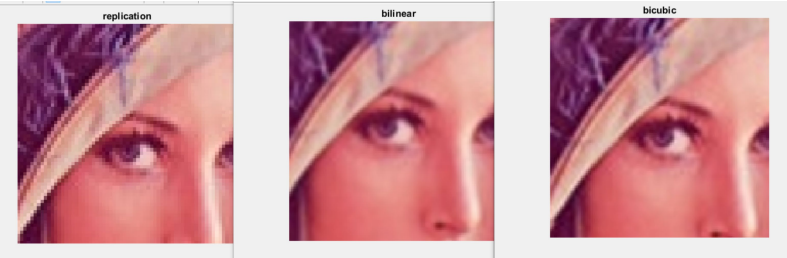
\includegraphics[keepaspectratio,alt={image.png}]{Lezione 2 Operazioni sulle matrici/image 4.png}}
\caption{image.png}
\end{figure}

\textbf{Cosa fare ai bordi?} Un \textbf{problema} è quello dei bordi:
come fare l'interpolazione ai bordi? Possibili soluzioni:

\begin{enumerate}
\def\labelenumi{\arabic{enumi}.}
\tightlist
\item
  Non fare nulla
\item
  Interpolare con i valori presenti anche se in numero minore di quelli
  usati per altri pixel.
\end{enumerate}

\textbf{Considerare solo le zone centrali dell'immagine:} in questo caso
non si calcolano i valori ai bordi.

\begin{figure}
\centering
\pandocbounded{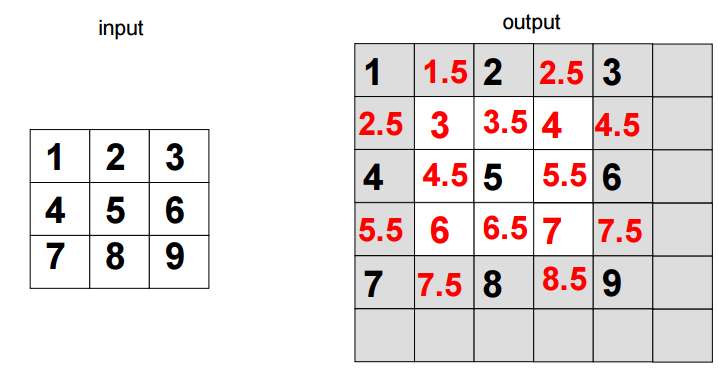
\includegraphics[keepaspectratio,alt={image.png}]{Lezione 2 Operazioni sulle matrici/image 5.png}}
\caption{image.png}
\end{figure}

Dopo aver fatto i calcoli replicare le ultime righe e colonne: in questo
caso per fare i calcoli si replicano semplicemente i valori nelle righe
e nelle colonne ``isolate''.

\begin{figure}
\centering
\pandocbounded{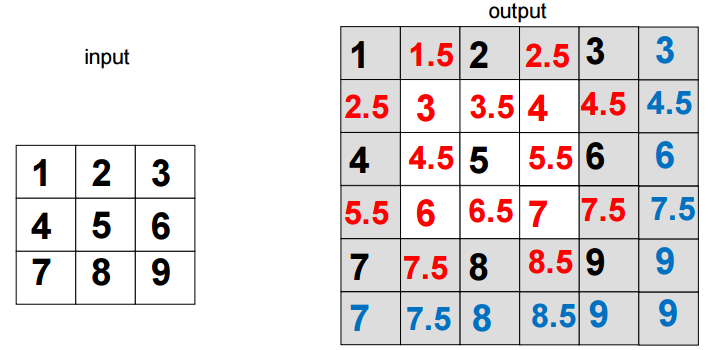
\includegraphics[keepaspectratio,alt={image.png}]{Lezione 2 Operazioni sulle matrici/image 6.png}}
\caption{image.png}
\end{figure}

\subsubsection{Zooming Out}\label{zooming-out}

Se lo zoom è fatto con un numero inferiore ad 1, si ottiene ovviamente
una immagine più piccola dell'originale, dato che di default la
dimensione dell'immagine originale corrisponde ad uno zoom pari ad 1.

Se riduco l'immagine, ho un processo detto di ``\textbf{decimazione}''.

Data una immagine \(m \times n\) con uno zooming out di 0,5, si otterrà
una immagine di \(m/2 \times n/2\).

\subsubsection{Decimazione}\label{decimazione}

\begin{itemize}
\item
  \textbf{Metodo 1} Ogni quattro pixel se ne sceglie uno.

  \begin{figure}
  \centering
  \pandocbounded{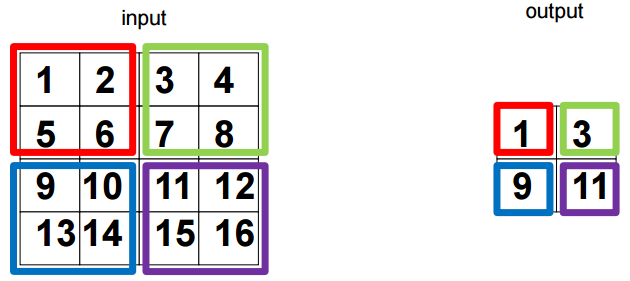
\includegraphics[keepaspectratio,alt={image.png}]{Lezione 2 Operazioni sulle matrici/image 7.png}}
  \caption{image.png}
  \end{figure}
\item
  \textbf{Metodo 2} Di quatto pixel se ne calcola il valore medio.
  Quindi si fa la somma dei pixel e si divide per il numero di essi. In
  questo caso si sommano i 4 pixel e si divide il risultato per 4.

  \begin{figure}
  \centering
  \pandocbounded{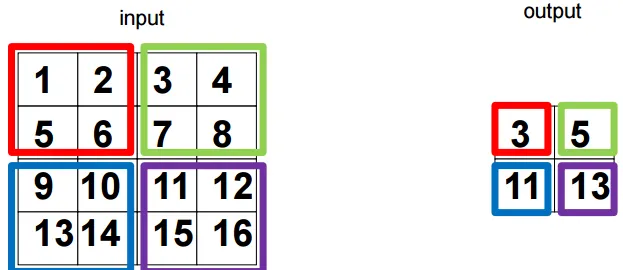
\includegraphics[keepaspectratio,alt={image.png}]{Lezione 2 Operazioni sulle matrici/48c87855-4e0c-43bf-ab3a-cc095c65499f.png}}
  \caption{image.png}
  \end{figure}
\end{itemize}

\subsubsection{Stima della qualità di un
algoritmo}\label{stima-della-qualituxe0-di-un-algoritmo}

Esistono 2 \textbf{algoritmi per stimare la qualità di un'immagine dopo
il processo di interpolazione e compressione} (ad esempio il passaggio a
JPEG).

Ci aiutano a misurare quanto un'immagine sia stata ``danneggiata''
alterata rispetto all'immagine originale denominata perfetta.

\begin{itemize}
\tightlist
\item
  \textbf{MSE (Mean Square Error - Errore Quadratico Medio)} L'MSE
  rappresenta la \textbf{distanza matematica pura} tra due immagini.
  Immagina di sovrapporre l'immagine originale (\(I\)) e quella
  modificata (\(I’\)) e di confrontare ogni singolo pixel nella stesso
  posizione \((x,y)\).
\end{itemize}

\textbf{Come funziona?} Per ogni coppia di pixel corrispondenti,
l'algoritmo calcola la differenza di intensità, la eleva al
\textbf{quadrato} (per rendere l'errore sempre positivo e ``punire''
maggiormente le differenze grandi) e infine calcola la \textbf{media} di
tutti questi quadrati sulla superficie dell'immagine \((M \times N)\).

\textbf{Significato del valore:} Più il valore dell'MSE è \textbf{vicino
allo zero}, maggiore è la fedeltà dell'immagine modificata rispetto
all'originale. Se l'MSE fosse zero, allora le due immagini sarebbero
identiche bit per bit.

\begin{verbatim}
$$
MSE = \frac{1}{MN} \sum_{x=1}^{M} \sum_{y=1}^{N} \left[ I'(x,y) - I(x,y) \right]^2
$$
\end{verbatim}

\begin{itemize}
\item
  \textbf{PSNR (Peak Signal to Noise Ratio - Rapporto segnale/rumore di
  picco)}

  Il \textbf{PSNR (Peak Signal to Noise Ratio)} è un parametro
  matematico utilizzato per \textbf{misurare la qualità di un'immagine}
  che ha subito un processo di modifica (come la compressione JPEG o
  l'ingrandimento) rispetto all'immagine originale.

  Immagina il PSNR come un punteggio di fedeltà. Per calcolarlo, devi
  obbligatoriamente confrontare due immagini: quella ``perfetta''
  originale e quella modificata.

  \textbf{Il rapporto tra ``Segnale'' e ``Rumore''} Il nome stesso ti
  dice cosa sta misurando:

  \begin{itemize}
  \tightlist
  \item
    \textbf{Peak Signal (Segnale di Picco):} rappresenta il valore
    massimo che un pixel può avere. Nelle immagini standard a 8 bit,
    questo valore è \textbf{255}.
  \item
    \textbf{Noise (Rumore):} rappresenta l'errore introdotto, ovvero la
    differenza tra i pixel dell'immagine originale e quella modificata.
    Questo errore viene calcolato tramite l'\textbf{MSE} (Errore
    Quadratico Medio).
  \end{itemize}

  L'algoritmo mette in rapporto questi due dati usando una scala
  logaritmica espressa in \textbf{decibel (dB)}.

  Come leggere il risultato

  A differenza dell'MSE (dove un valore basso è positivo), per il
  \textbf{PSNR vale la regola: più è alto, meglio è}.

  \begin{itemize}
  \tightlist
  \item
    Un \textbf{PSNR elevato} indica che l'immagine modificata è molto
    simile all'originale (alta qualità).
  \item
    Un \textbf{PSNR basso} indica che c'è molta differenza (distorsione)
    e quindi la qualità è scarsa.
  \end{itemize}

  \textbf{Perché si usa il logaritmo?}

  Si utilizza una scala logaritmica perché la percezione umana
  dell'intensità luminosa non è lineare, ma segue appunto una funzione
  logaritmica. Il PSNR cerca quindi di trasformare un errore numerico in
  un valore che si avvicini (anche se in modo imperfetto) alla
  sensibilità dell'occhio.

  \textbf{I limiti (Cosa il PSNR ``non vede'')} Nonostante sia il
  parametro più diffuso, il PSNR ha dei difetti importanti legati al
  sistema visivo umano (\textbf{HVS}):

  \begin{itemize}
  \tightlist
  \item
    \textbf{Sensibilità spaziale:} Se sposti un'immagine di un solo
    pixel (traslazione) o la ruoti leggermente, per l'occhio umano
    l'immagine è identica, ma per il PSNR il punteggio crolla
    drasticamente perché i pixel non corrispondono più matematicamente
    nella griglia.
  \item
    \textbf{Mancanza di contesto:} Il PSNR tratta ogni errore allo
    stesso modo, mentre l'occhio umano è più o meno sensibile agli
    errori a seconda che si trovino in zone chiare, scure o con molti
    dettagli.
  \end{itemize}

  \textbf{In sintesi:} \textbf{Il PSNR trasforma la ``distanza''
  matematica tra due immagini (l'errore MSE) in un indice di qualità
  espresso in decibel.} Se stai comprimendo una foto e il PSNR aumenta,
  significa che stai facendo un buon lavoro e che l'immagine finale è
  più \textbf{``fedele''} all'originale.

  \[
    PSNR = -10 \log_{10} \frac{MSE}{S^2}
    \\
    \\
    PSNR = 20 \log_{10} \left( \frac{S}{\sqrt{MSE}} \right)
    \\
    \\
    PSNR = 10 \log_{10} \left( \frac{S^2}{MSE} \right)
    \]
\end{itemize}
